\documentclass[9pt]{beamer}
%\makeatletter
%\def\beamer@calltheme#1#2#3{%
%	\def\beamer@themelist{#2}
%	\@for\beamer@themename:=\beamer@themelist\do
%	{\usepackage[{#1}]{\beamer@themelocation/#3\beamer@themename}}}
%
%\def\usefolder#1{
%	\def\beamer@themelocation{#1}
%}
%\def\beamer@themelocation{}

%\usefolder{../config}

\usetheme[
block=fill,
titleformat=regular,
progressbar=frametitle
]{metropolis}
%\metroset[everytitleformat=regular] % regular, lowercase, uppercase ]
%\metroset[inner/block=fill]

%\setbeameroption{show notes} 
\usepackage{booktabs}
\usepackage[scale=2]{ccicons}

\usepackage{pgfplots}
\usepgfplotslibrary{dateplot}


%\ Hrvatski znakovi
\usepackage[utf8]{inputenc}
\usepackage[T1]{fontenc}
\usepackage[croatian]{babel}
\usepackage{todonotes}
\usepackage{amsmath}
\usepackage{amsfonts}
\selectlanguage{croatian} % american ngerman
\usepackage{todonotes}

% Koristenje Latin modern fonta
% Bez toga na nekim racunalima baca
% err: Font <taj i taj> at <mala velicina, npr4.0pt> not loadable: Metric (TFM) file not found. \end{frame}
\usepackage{lmodern}


\definecolor{RoyalBlue}{cmyk}{1, 0.50, 0, 0}
%\usepackage{natbib}
%\usepackage{bibentry}
\usepackage{scrextend}
\usepackage{hyperref}
%\usepackage[pdfa=true]{hyperref}
\hypersetup{%
    %draft, % = no hyperlinking at all (useful in b/w printouts)
    %colorlinks=true, 
    linktocpage=true, pdfstartpage=3, pdfstartview=FitV,%
    % uncomment the following line if you want to have black links (e.g., for printing)
    %colorlinks=false, linktocpage=false, pdfborder={0 0 0}, pdfstartpage=3, pdfstartview=FitV,% 
    breaklinks=true, pdfpagemode=UseNone, pageanchor=true, pdfpagemode=UseOutlines,%
    plainpages=false, bookmarksnumbered, bookmarksopen=true, bookmarksopenlevel=1,%
    hypertexnames=true, pdfhighlight=/O,%nesting=true,%frenchlinks,%
    %urlcolor=webbrown, linkcolor=RoyalBlue, citecolor=webgreen, %pagecolor=RoyalBlue,%
    %urlcolor=Blue, linkcolor=Blue, citecolor=Red, %pagecolor=Black,%
    %pdftitle={\myTitle},%
    %pdfauthor={\textcopyright\ \myName, \myUni, \myFaculty},%
    pdfsubject={},%
    pdfkeywords={},%
    pdfcreator={pdfLaTeX},%
    pdfproducer={LaTeX with hyperref and classicthesis}, %
    unicode = true 
} 

%\usepackage[pdftex]{graphicx}
% declare the path(s) where your graphic files are
\graphicspath{{./}{./figures/}}


\newcommand{\executeiffilenewer}[3]{%
	\ifnum\pdfstrcmp{\pdffilemoddate{#1}}%
	{\pdffilemoddate{#2}}>0%
	{\immediate\write18{#3}}\fi%
}
\newcommand{\includesvg}[1]{%
	\executeiffilenewer{#1.svg}{#1.pdf}%
	{inkscape -z -C --file=#1.svg %
		--export-pdf=#1.pdf --export-latex}%
	\input{#1.pdf_tex}%
}


% http://tex.stackexchange.com/questions/83882/how-to-highlight-python-syntax-in-latex-listings-lstinputlistings-command

\usepackage{listings}
\usepackage{color}
\usepackage[semibold]{sourcecodepro}

% Default fixed font does not support bold face
\DeclareFixedFont{\ttb}{T1}{txtt}{bx}{n}{12} % for bold
\DeclareFixedFont{\ttm}{T1}{txtt}{m}{n}{12}  % for normal
% Custom colors
\definecolor{deepblue}{rgb}{0,0,0.5}
\definecolor{deepred}{rgb}{0.6,0,0}
\definecolor{deepgreen}{rgb}{0,0.5,0}


% Python style for highlighting
\newcommand\pythonstyle{\lstset{
		language=Python,
		basicstyle=\small\ttfamily,
		otherkeywords={self},             % Add keywords here
		keywordstyle=\small\ttfamily\color{deepblue},
		emph={MyClass,__init__},          % Custom highlighting
		emphstyle=\small\ttfamily\color{deepred},    % Custom highlighting style
		stringstyle=\color{deepgreen},
		frame=tb,                         % Any extra options here
		showstringspaces=false            % 
	}}
	
	
	% Python environment
	\lstnewenvironment{python}[1][]
	{
		\pythonstyle
		\lstset{#1}
	}
	{}
	
	% Python for external files
	\newcommand\pythonexternal[2][]{{
			\pythonstyle
			\lstinputlisting[#1]{#2}}}
	
	% Python for inline
	\newcommand\pythoninline[1]{{\pythonstyle\lstinline!#1!}}
%\documentclass[ucs]{beamer}
%\usetheme[menuwidth={0.3\paperwidth}]{erlangen}
%\setbeamercovered{transparent=20} 

\usepackage{amsmath,amsfonts,amsthm,amssymb}
\usepackage{setspace}
\usepackage{Tabbing}
\usepackage{fancyhdr}
\usepackage{lastpage}
\usepackage{extramarks}
\usepackage{chngpage}
\usepackage{soul,color}
\usepackage{graphicx,float,wrapfig}
\usepackage{xcolor}
\usepackage[normalem]{ulem}
\usepackage{mathtools}
\usepackage{cancel}

\definecolor{erlangenlyellow}{RGB}{123, 25, 121}
%\usepackage[utf8x]{inputenc}
%\usepackage{default}
%\usepackage[T1]{fontenc}

\usepackage{verbatim}
\usepackage{listings}
\usepackage{algorithm2e}


\usepackage{subcaption}
\usepackage{lmodern}

\title{Ray tracing, nastavak}

\subtitle{Ray tracing is the future and ever will be\ldots - David Kirk}
\institute{Računalna grafika}

\begin{document}
\begin{frame}
	\titlepage
\end{frame}

\begin{frame}{Sadržaj}
\tableofcontents
% You might wish to add the option [pausesections]
\end{frame}
\section{Vanjska ili unutrašnja strana?}
\begin{frame}{Vanjska ili unutrašnja strana?}
\begin{figure}
	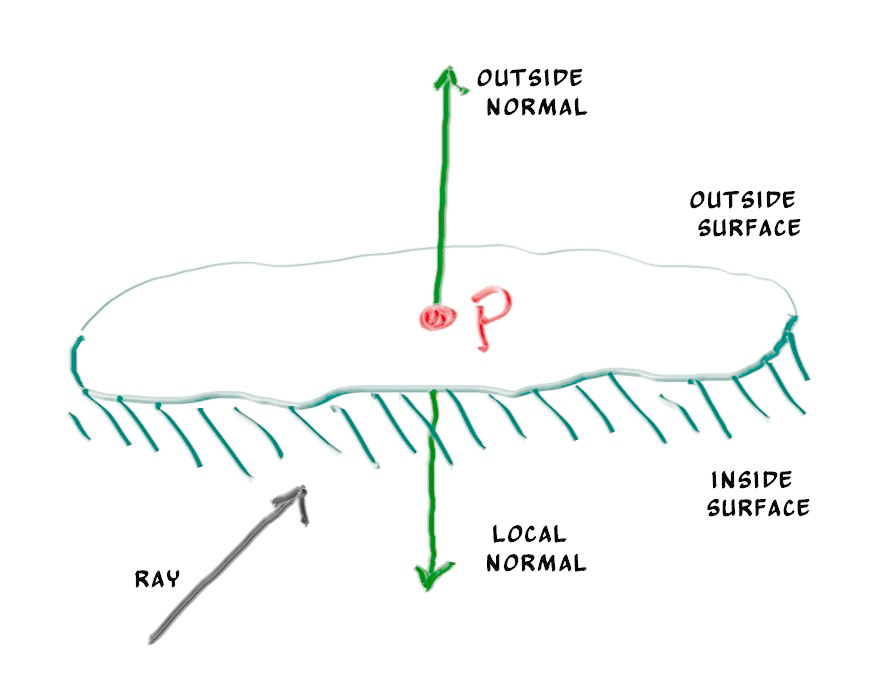
\includegraphics[width=0.5\textwidth]{./slike/normal-possibilities.png}
\end{figure}
\begin{itemize}
	\item Odredimo varijablu koja nam označava \textit{stranu}
	\item $\mathbf{D}\cdot \vec{n} >0$ zraka je s unutarnje strane
	\begin{itemize}
		\item \textit{okrećemo smjer} normale: $\vec{n} = -\vec{n}$
	\end{itemize}
	\item $\mathbf{D}\cdot \vec{n} <0$ zraka je s vanjske strane
\end{itemize}
\end{frame}

\section{Antialiasing}
\begin{frame}{Antialiasing}
\begin{figure}
	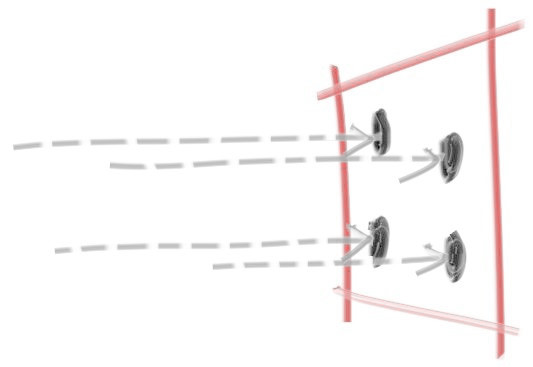
\includegraphics[width=0.3\textwidth]{./slike/pixel-samples.png}
	\caption{Uzorkovanje po pikselu}
\end{figure}
\begin{algorithm}[H]
	% \SetAlgoLined
	\ForEach{pixel, i,j}
	{
		pixelColor=(0, 0,0)\;
		\For{s<sampleNum; s++}
		{
			u = (i + rand()) / (imgw-1)\;
			v = (j + rand()) / (imgh-1)\;
			ray r(u,v)\;
			pixelColor += rayColor(r);
		}
		pixelColor /= sampleNum;
	}
	%\caption{How to write algorithms}
\end{algorithm}
\end{frame}

\begin{frame}{Difuzni materijali}
\begin{figure}
	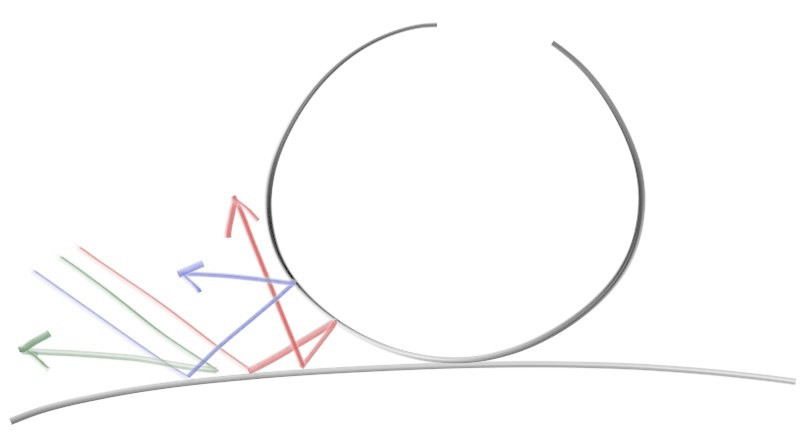
\includegraphics[width=0.5\textwidth]{./slike/light-bounce.png}
	\caption{Kako se odbijaju zrake od difuznih površina}
\end{figure}
Umjesto računanja $\vec{n}\cdot \vec{l}$:
\begin{itemize}
	\item Kreira se $N_{childRays}$ zraka koje se nasumično odbijaju od površine
\end{itemize}
\end{frame}

\begin{frame}{Difuzni materijali, generiranje nasumične zrake, intuitivni pristup}
\begin{figure}
	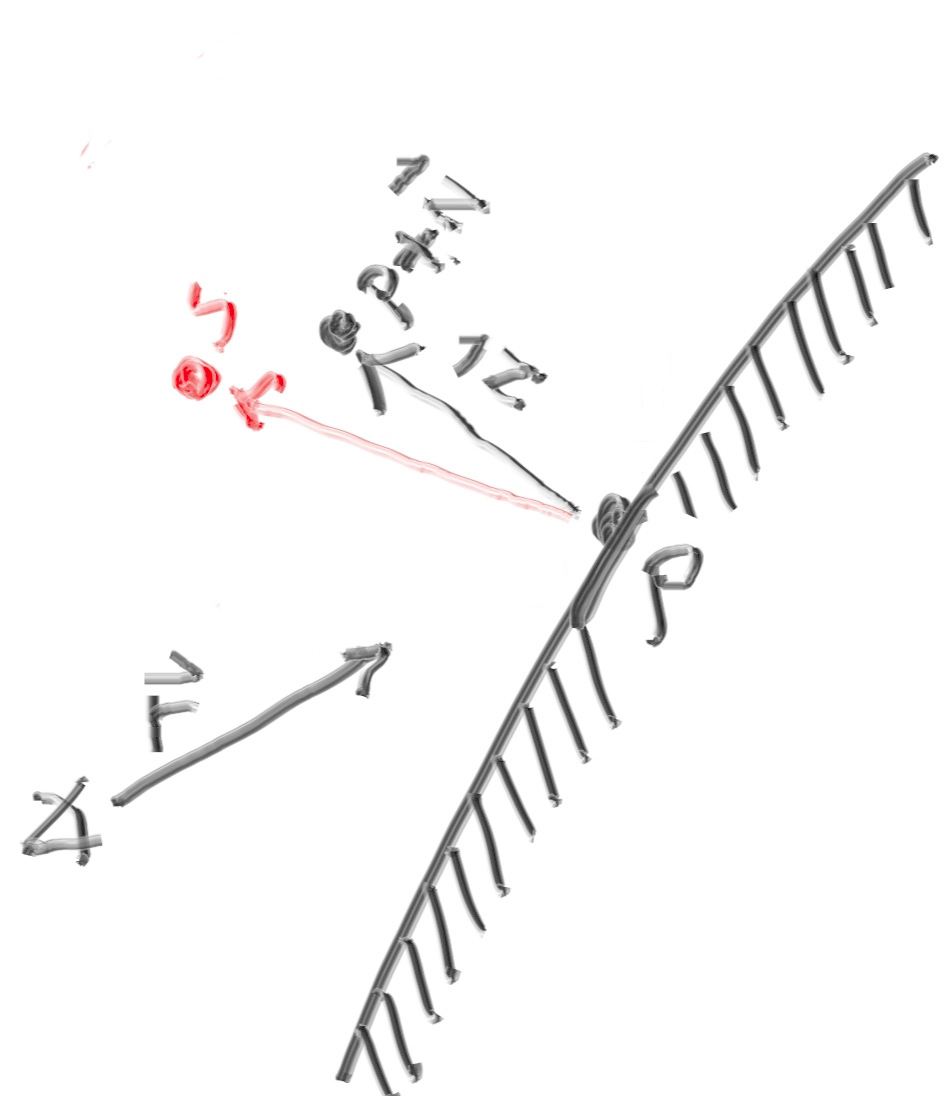
\includegraphics[width=0.2\textwidth]{./slike/rand-vector2.png}
	\caption{Jedinična kugla}
\end{figure}

\begin{itemize}
	\item Odrediti nasumičnu točku $\mathbf{S}$, $s$ je $\mathbb{R} \cap \left[-1, 1\right]$ 
	\item $\mathbf{S} = \mathbf{P} + \vec{n} + (s_1, s_2, s_3)$
%	\item  $\mathbf{D} = \mathbf{S}-\mathbf{P}$
\end{itemize}
\end{frame}

\begin{frame}{Difuzni materijali, generiranje nasumične zrake, skoro kao prije}
\begin{figure}
	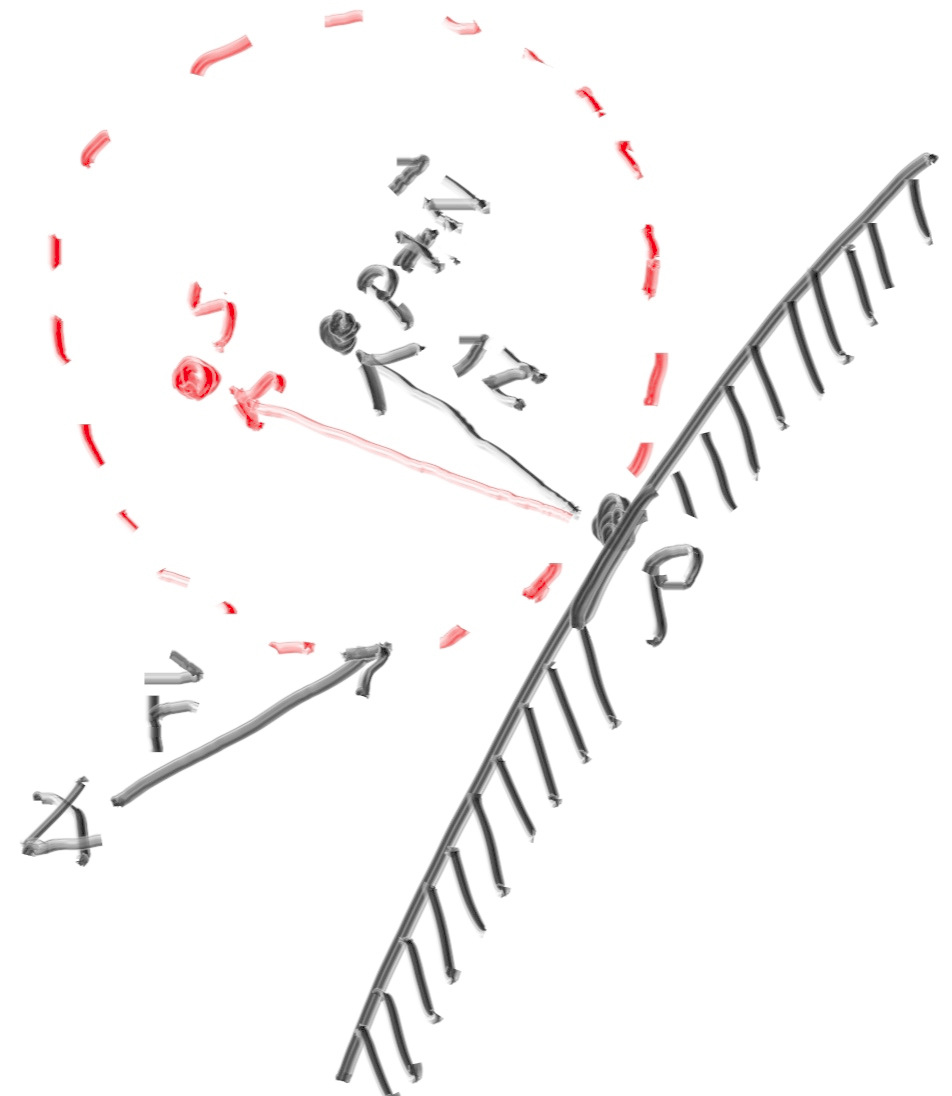
\includegraphics[width=0.2\textwidth]{./slike/rand-vector.png}
	\caption{Jedinična kugla}
\end{figure}
\begin{itemize}
	\item Odrediti središte kugle: $\mathbf{P} + \vec{n}$
	\item Odrediti nasumičnu točku $\mathbf{S}$ \textbf{unutar} kugle
	\begin{itemize}
		\item Odrediti nasumičnu točku $\mathbf{S}'(x,y,z)$u jediničnoj kocki $x, y, z \in \left[-1, 1\right]$
		\item Provjerimo je li ta točka unutar kugle, onda \item $\mathbf{S} = \mathbf{P} + \vec{n} + (x, y, z)$
		\item Odbacimo ako nije, ili ako vrijedi $||\mathbf{S}'|| \geq 1$
	\end{itemize}
	\item Odrediti vektor smjera $\mathbf{D}$ zrake: $\mathbf{D} = \mathbf{S}-\mathbf{P}$
	\item Kreiramo novu zraku i provjerimo siječe li se s kojim objektom
	\item Treba nam \textit{limit} kada prestajemo s generiranjem rekurzivnih zraka
	\item Za svaku zraku zbrajamo doprinos boje
\end{itemize}
\end{frame}

\begin{frame}{Difuzni materijali, generiranje nasumične zrake, malo bolje}
\begin{figure}
	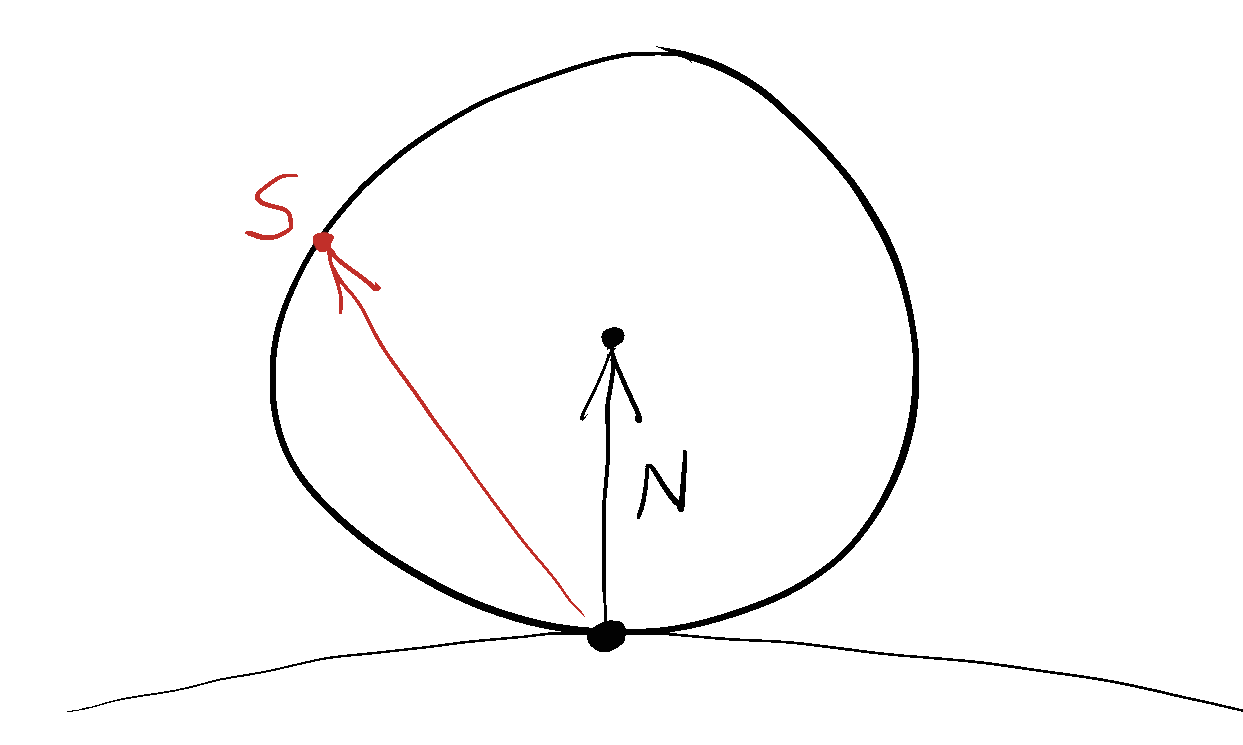
\includegraphics[width=0.3\textwidth]{./slike/rand-unitvector.png}
	\caption{Nasumična točka na sferi kugle}
\end{figure}
Sve je isto kao i prije, ali:
\begin{itemize}
	\item Odrediti nasumičnu točku $\mathbf{S}$ na \textbf{sferi} kugle
	\item $a$ je $\mathbb{R} \cap \left[0, 2\pi\right]$, $z$ je $\mathbb{R} \cap \left[-1, 1\right]$, $r = \sqrt{1-z^2}$
	\item $\mathbf{S} = (r\cos a, r\sin a, z)$
\end{itemize}
Rezultat:
\begin{itemize}
	\item Mekše sjene  
\end{itemize}
\end{frame}
\section{Materijali i Refleksija}
\begin{frame}{Refleksija}
\begin{figure}
	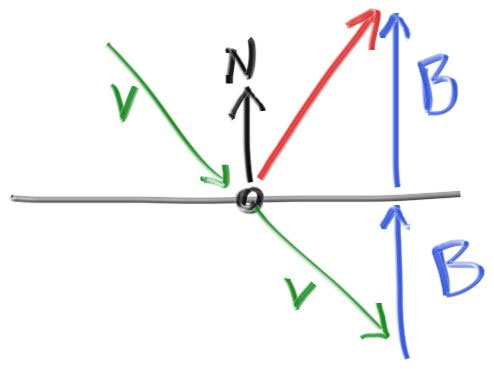
\includegraphics[width=0.3\textwidth]{./slike/ray-reflect.png}
	\caption{Refleksija}
\end{figure}
\begin{itemize}
	\item $\mathbf{B} = \mathbf{v}\cdot\vec{n}$
	\item $\mathbf{r} = \mathbf{D} - 2\mathbf{B}\vec{n} $
	\item Odredimo boju materijala $\vec{c}$
	\item Pratimo zraku u smjeru $\mathbf{r}$
	\item Izračunamo boju koju generira ta zraka	
	\item Ako je materijal difuzan, radimo kao i prije, samo množimo dobivenu boju(svih raspršenih zraka) s bojom materijala $\vec{c}$
\end{itemize}
\end{frame}
\begin{frame}{Refleksija, zašto samo jedna zraka?}
\begin{figure}
	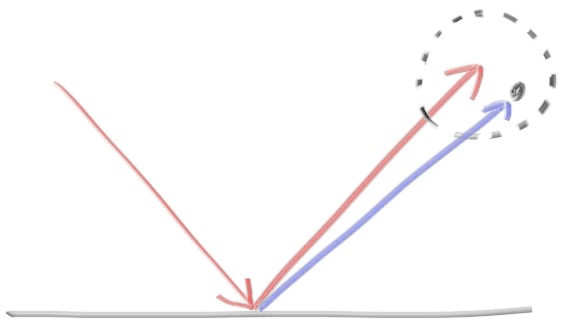
\includegraphics[width=0.3\textwidth]{./slike/reflect-fuzzy.png}
	\caption{Zrake u dominantno refleksivnom smjeru}
\end{figure}
\begin{itemize}
	\item Radimo kao i sa idealno difuznim materijalom, ali
	\begin{itemize}
		\item Odašiljemo nasumične zrake unutar kugle proizvoljnog radijusa
		\item Što je veći radijus kugle, refleksija je zamućenija
	\end{itemize}
\end{itemize}
\end{frame}
\section{Refrakcija}
\begin{frame}{Refrakcija}
\begin{figure}
	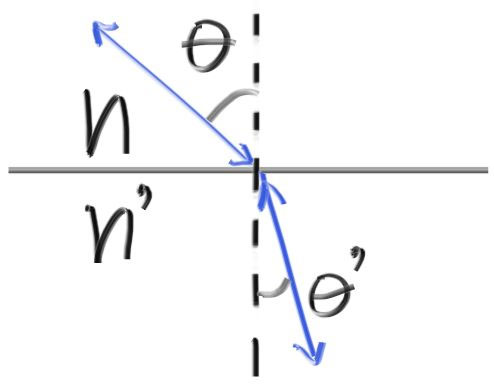
\includegraphics[width=0.3\textwidth]{./slike/ray-refract.png}
	\caption{Refrakcija}
\end{figure}
\begin{columns}
	\begin{column}{0.5\linewidth}
		Ponavljanje:
		\begin{itemize}
			\item $\eta \sin \theta= \eta' \sin \theta'$
			\item $\sin \theta' = \frac{\eta}{\eta'}\sin \theta $
			\item $\mathbf{R'} =\mathbf{R'}_{\parallel} + \mathbf{R'}_{\bot}$
			\item $\mathbf{R'}_{\parallel} = \frac{\eta}{\eta'} (\mathbf{R} + \cos\theta \mathbf{n})$
			\item $\mathbf{R'}_{\bot} = -\sqrt{1 - |\mathbf{R'}_{\parallel}|^2} \mathbf{n}$
			\item $\mathbf{R'}_{\parallel} =
			\frac{\eta}{\eta'} (\mathbf{R} + (\mathbf{-R} \cdot \mathbf{n}) \mathbf{n})$
		\end{itemize}
	\end{column}
	\begin{column}{0.5\linewidth}
		\begin{itemize}
			\item Sada samo moramo pratiti zraku dalje \ldots
		\end{itemize}
	\end{column}
\end{columns}

\end{frame}
\begin{frame}{Problem}
\begin{itemize}
	\item $\sin \theta' = \frac{\eta}{\eta'}\sin \theta $
	\item ako je $\eta > \eta'$
	\item Može se desiti da $\sin \theta' > 1$, a to ne smijemo dopustiti
	\item U tom slučaju, zraka se mora reflektirati, nema refrakcije
	\item Obično je takva situacija unutar nekog objekta, tada se to naziva \textit{potpuna unutarnja refleksija}
\end{itemize}
\end{frame}

\begin{frame}{Refrakcija, refleksija ovise o kutu gledanja}

\begin{align*}
	R(\theta) &= R_0 + (1-R_0)(1-\cos\theta)^5 \\
	R_0 &= \left(\frac{\eta - \eta'}{\eta + \eta'}\right)^2
\end{align*}
\begin{itemize}
	\item $\theta$ kut između zrake i normale površine $\cos\theta = \vec{n}\cdot\mathbf{v}$
	\item R je koeficijent refleksije
\end{itemize}
\end{frame}

\section{Unutar ili izvan fokusa?}
\begin{frame}{Jasno, još zraka}
\begin{figure}
	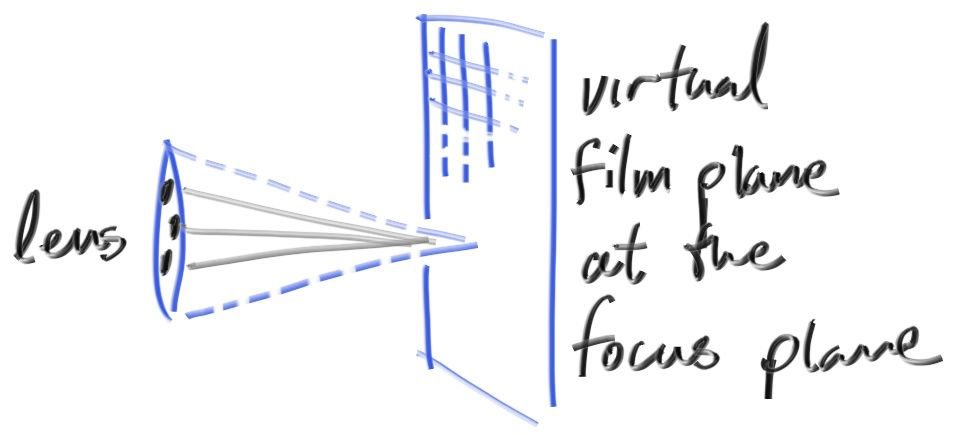
\includegraphics[width=0.5\textwidth]{./slike/cam-film-plane.png}
	\caption{Aproksimacija \textit{focus blur}}
\end{figure}
\begin{itemize}
	\item Ne odašiljemo zrake samo iz jedne točke, već
	\item iz diska(kružnica) proizvoljnog radijusa 
\end{itemize}
\end{frame}
\plain{Ptanja?}
\end{document} 
